\documentclass[a4j]{jarticle}

\usepackage[dvipdfmx]{graphicx}
\usepackage{url}
\usepackage{here}
%\usepackage{listings}
\usepackage{amsmath,amssymb}
\usepackage[dvipdfmx]{color}

\setlength{\headsep}{-5mm}
\setlength{\oddsidemargin}{0mm}
\setlength{\textwidth}{165mm}
\setlength{\textheight}{230mm}
\setlength{\footskip}{20mm}

\title{
\vspace{30mm}
{\bf 子育て支援システム}
\\
\vspace{5mm}
{\bf 内部設計書v1\\
}
\vspace{120mm}
}

\author{
\vspace{5mm}
チーム名 007\\
\vspace{5mm}
}


\begin{document}
\maketitle
\tableofcontents
\newpage


\subsection{ゲーム機能}
\subsubsection{ゲーム選択画面\label{ゲーム選択}}
\begin{figure}[H]
    \begin{center}
    \resizebox{16.5cm}{!}{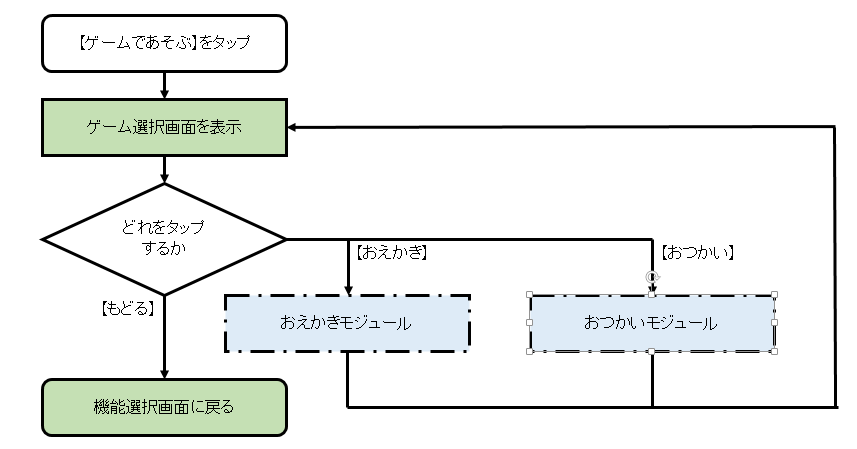
\includegraphics {ゲーム_全体.PNG}}
    \caption {ゲーム選択モジュールのイメージ}
    \label{functionselection}
    \end{center}
\end{figure}

\subsubsection*{概要}
 利用者が行うゲームを選択する画面です。

\subsubsection*{処理フロー}
\begin{itemize}
\item 【おえかき】をタップすることでおえかき選択モジュールを呼び出します。
\item 【おつかい】をタップすることでおつかいモジュールを呼び出します。
\item 【もどる】をタップすることで機能選択画面(第\ref{機能選択}節)に戻ります。
\item
\end{itemize}

\newpage
\subsection{おえかき選択モジュール}
\subsubsection{おえかき選択画面\label{おえかき選択}}
\begin{figure}[H]
    \begin{center}
    \resizebox{16.5cm}{!}{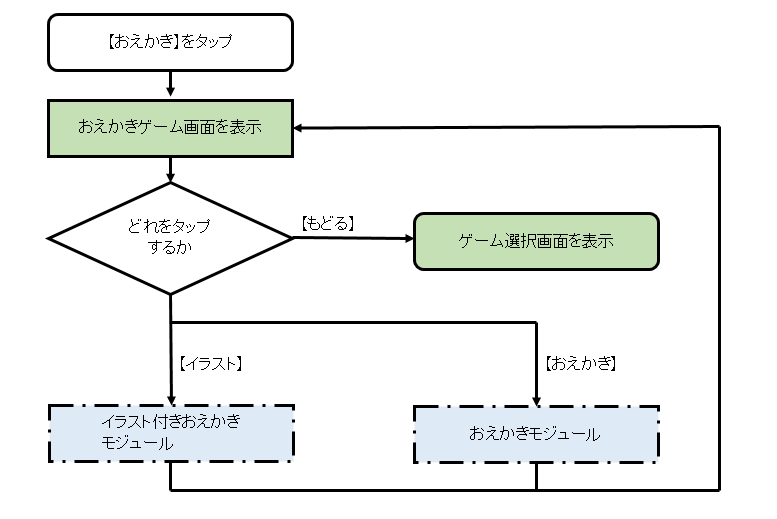
\includegraphics {ゲーム_おえかき.PNG}}
    \caption {おえかき選択モジュールのイメージ}
    \label{functionselection}
    \end{center}
\end{figure}

\subsubsection*{概要}
 おえかきの種類を選択する画面です。

\subsubsection*{処理フロー}
\begin{itemize}
\item 【イラスト】をタップすることでイラスト付きおえかきモジュールを呼び出します。
\item 【おえかき】をタップすことでおえかきモジュールを呼び出します。
\item 【もどる】をタップすることでゲーム選択画面(第\ref{ゲーム選択}節)に戻ります。
\end{itemize}

\newpage
\subsection{おえかきモジュール}
\subsubsection{おえかき画面\label{おえかき}}
\begin{figure}[H]
    \begin{center}
    \resizebox{16.5cm}{!}{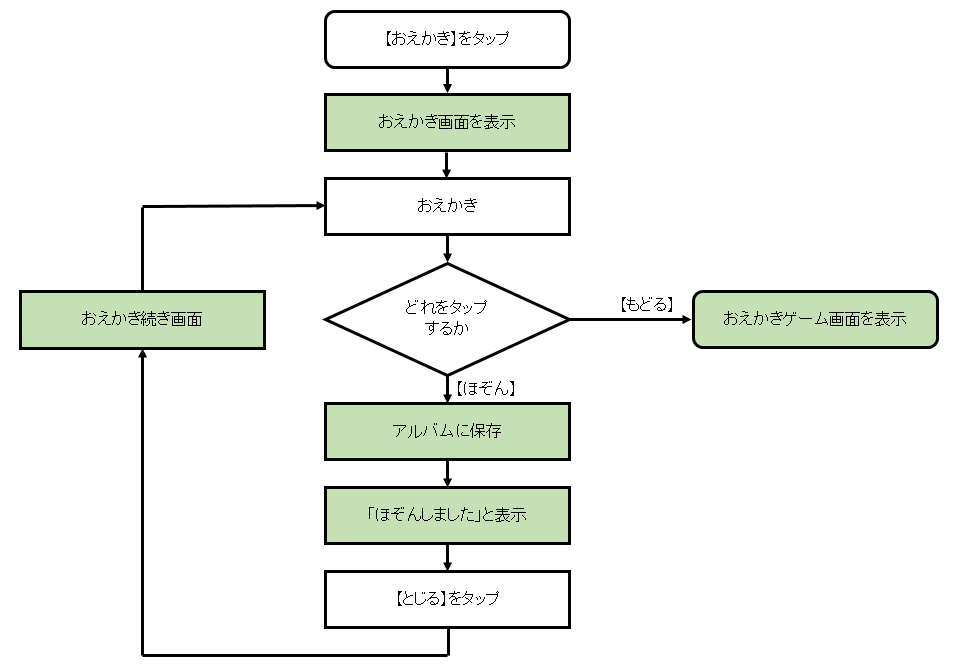
\includegraphics {ゲーム_おえかき2.PNG}}
    \caption {おえかきモジュールのイメージ}
    \label{functionselection}
    \end{center}
\end{figure}

\subsubsection*{概要}
 利用者が実際におえかきゲームで遊ぶための画面です。\\
機能としておえかきを描いたり、描いたおえかきを成長記録のアルバムに保存することができます。
\subsubsection*{処理フロー}
\begin{itemize}
\item 【イラスト】をタップすることでおえかきをするためのペンやペンの太さ、消しゴム、色の種類を変更できます。
\item 【ほぞん】をタップすことで自分の描いたおえかきが成長記録のアルバムに保存されます。
\item 【もどる】をタップすることでおえかき選択モジュール(第\ref{おえかき選択}節)に戻ります。
\end{itemize}

\newpage
\subsection{イラスト付きおえかきモジュール}
\subsubsection{イラスト付きおえかき画面\label{イラスト}}
\begin{figure}[H]
    \begin{center}
    \resizebox{16.5cm}{!}{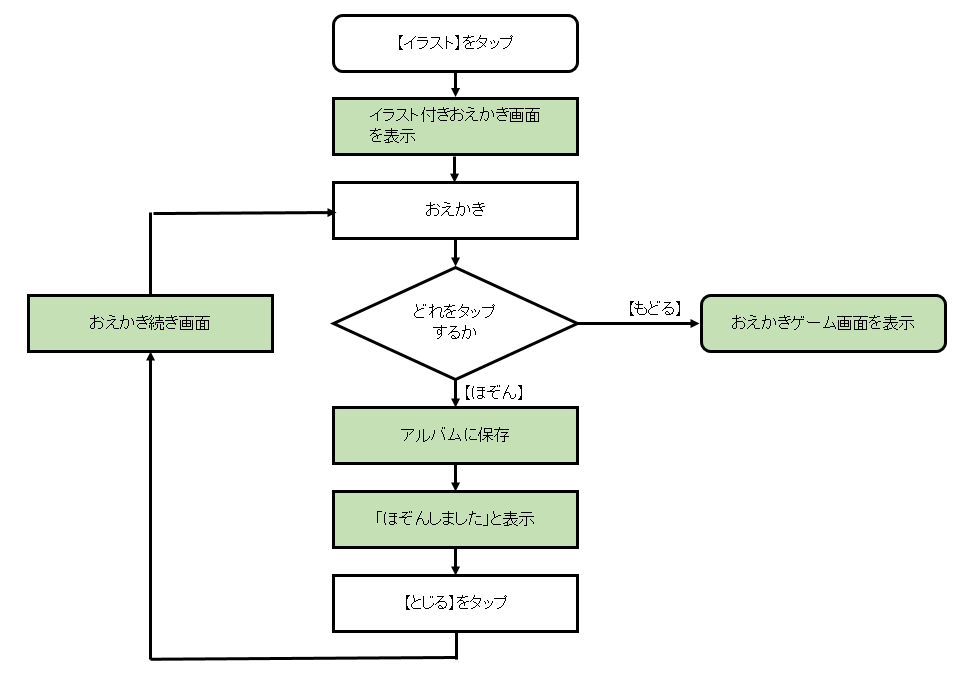
\includegraphics {ゲーム_イラスト.PNG}}
    \caption {イラスト付きおえかきモジュールのイメージ}
    \label{functionselection}
    \end{center}
\end{figure}

\subsubsection*{概要}
利用者が実際におえかきゲームで遊ぶための画面です。\\
機能として用意されたイラストを閲覧しながらおえかきを描いたり、描いたおえかきを成長記録のアルバムに保存することができます。

\subsubsection*{処理フロー}
\begin{itemize}
\item 【イラスト】をタップすることでおえかきをするためのペンやペンの太さ、消しゴム、色の種類を変更できます。
\item 【ほぞん】をタップすことで自分の描いたおえかきが成長記録のアルバムに保存されます。
\item 【もどる】をタップすることでおえかき選択モジュール(第\ref{おえかき選択}節)に戻ります。
\end{itemize}


\newpage
\subsection{おつかいモジュール}
\subsubsection{おつかい画面\label{おつかい}}
\begin{figure}[H]
    \begin{center}
    \resizebox{16.5cm}{!}{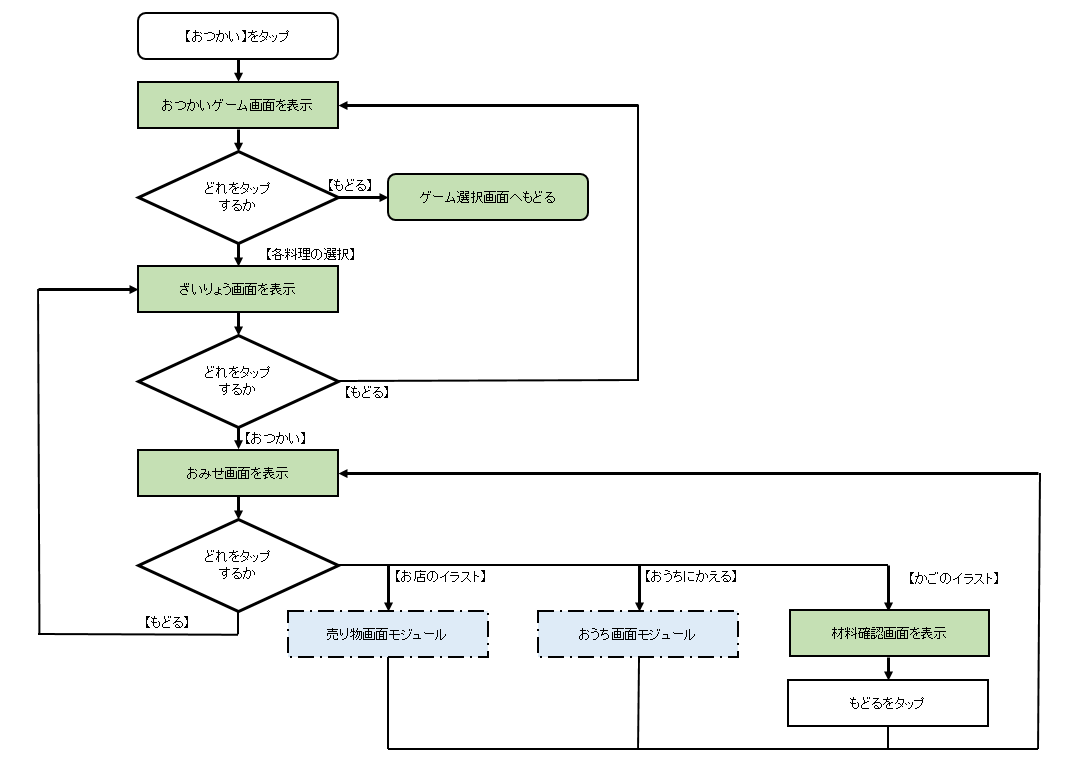
\includegraphics {ゲーム_おつかい.PNG}}
    \caption {おつかいモジュールのイメージ}
    \label{functionselection}
    \end{center}
\end{figure}

\subsubsection*{概要}
利用者が実際におつかいゲームで遊ぶための画面です。\\
機能は選択した料理の材料を買ってくるゲームです。

\subsubsection*{処理フロー}
\begin{itemize}
\item 【もどる】をタップすることでゲーム選択画面(第\ref{ゲーム選択}節)に戻ります。
\item 【各料理】をタップすることで選択した勝利の材料画面を表示します。
\item 材料画面の【おつかい】をタップするとおみせ画面を表示し、【もどる】をタップするとおつかいゲーム画面を表示します。
\item 【お店のイラスト】をタップすることで売り物画面モジュール(第\ref{売り物}節)を呼び出します。
\item 【おうちにかえる】をタップすることでおうち画面モジュール(第\ref{おうち}節)を呼び出します。
\item 【かごのイラスト】をタップすることで材料確認画面に遷移し持っている材料を確認できます。
\end{itemize}


\newpage
\subsection{売り物モジュール}
\subsubsection{売り物モジュール\label{売り物}}
\begin{figure}[H]
    \begin{center}
    \resizebox{16.5cm}{!}{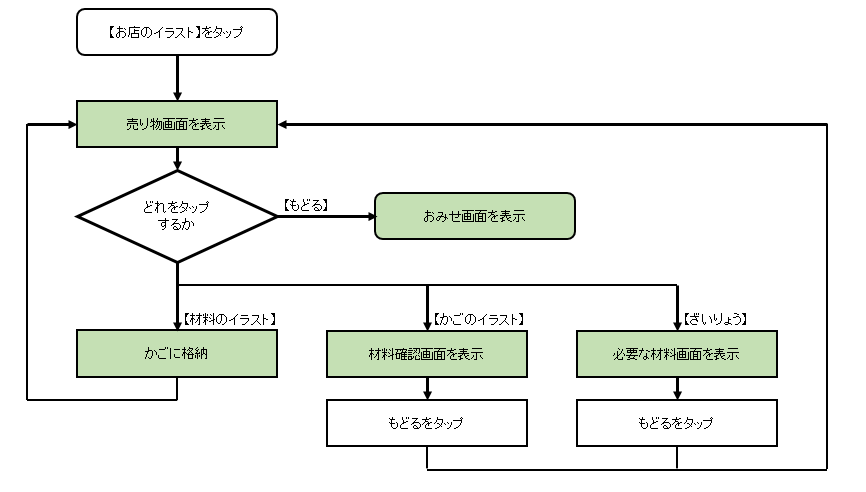
\includegraphics {ゲーム_おつかい_売り物.PNG}}
    \caption {おつかいモジュールのイメージ}
    \label{functionselection}
    \end{center}
\end{figure}

\subsubsection*{概要}
おつかいゲームの売り物画面へ遷移後の処理を行います。\\
ここでは、必要な材料を買うことができます。

\subsubsection*{処理フロー}
\begin{itemize}
\item 【もどる】をタップすることでおみせ画面に戻ります。
\item 【材料のイラスト】をタップすることでかごにタップした材料が格納されます。
\item 【かごのイラスト】をタップすることで材料確認画面に遷移し持っている材料を確認できます。
\item 【ざいりょう】をタップすることで料理に必要な材料を表示します。
\end{itemize}

\newpage
\subsection{おうちモジュール}
\subsubsection{おうちモジュール\label{おうち}}
\begin{figure}[H]
    \begin{center}
    \resizebox{16.5cm}{!}{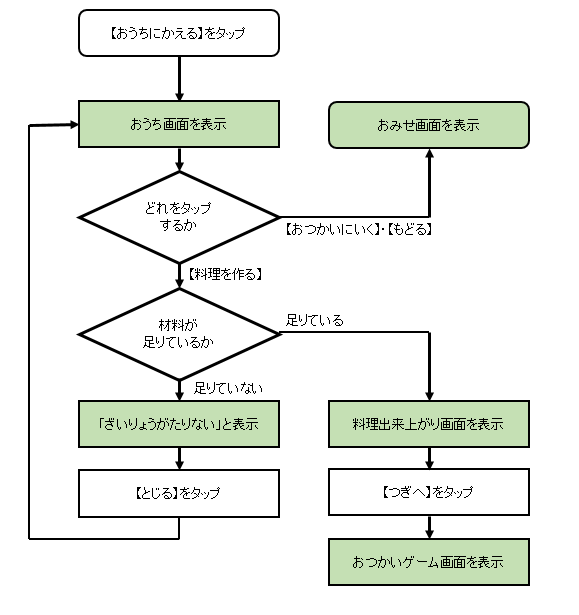
\includegraphics {ゲーム_おつかい_おうち.PNG}}
    \caption {おうちモジュールのイメージ}
    \label{functionselection}
    \end{center}
\end{figure}

\subsubsection*{概要}
おつかいのおうち画面に遷移後の処理を行います。\\
ここでは、おつかい画面で選択した料理を持っている材料で作ることができます。

\subsubsection*{処理フロー}
\begin{itemize}
\item 【おつかいにいく】・【もどる】をタップすることでおみせ画面に戻ります。
\item 【料理を作る】をタップすると材料が足りている場合と足りてない場合に分岐します。足りている場合は出来上がり画面を表示し、足りてない場合は「ざいりょうがたいない」と表示します。
\item 足りている時に表示された画面の【つぎへ】をタップすることでおつかいゲーム画面に戻ります。
\item 足りていない時に表示された画面の【とじる】をタップすることでおうち画面へ遷移します。
\end{itemize}

\end{document}
